حصہ{خطی تخمین اور تفرقات}
بعض اوقات پیچیدہ تفاعل کو سادہ تخمینی تفاعل سے  ظاہر کرتے ہوئے مخصوص موقعوں پر قابل قبول نتائج حاصل کرنا ممکن ہوتا ہے۔ ان سادہ تفاعل کے ساتھ کام کرنا زیادہ آسان ثابت ہوتا ہے۔ اس حصہ میں مماس پر مبنی \اصطلاح{خطی صورتوں}\حاشیہب{linearizations} پر غور کیا گیا ہے۔

ہم نئے متغیرات \عددی{\dif x} اور \عددی{\dif y} متعارف کرتے ہیں جو \عددی{\tfrac{\dif y}{\dif x}} کو نئی معنی دیں گے۔  ہم تجرباتی پیمائش میں خلل اور حساسیت  کو \عددی{\dif y} سے ظاہر کریں گے۔

\جزوحصہء{خطی تخمین}
آپ شکل \حوالہ{شکل_استعمال_منحنی_اور_مماس} میں دیکھ سکتے ہیں کہ منحنی \عددی{y=f(x)} کا مماس نقطہ مماس کے نزدیک منحنی کے قریب رہتا ہے۔نقطہ مماس کے دونوں اطراف چھوٹے وقفہ پر مماس کی \عددی{y} قیمت کو  منحنی کی \عددی{y} تخمینی قیمت تصور کیا جا سکتا ہے۔
\begin{figure}
\centering
\begin{subfigure}{0.5\textwidth}
\centering
\begin{tikzpicture}[font=\small]
\begin{axis}[small,axis lines=middle,xlabel={$x$},ylabel={$y$}]
\addplot[domain=-1:2]{x^2}node[pos=0.9,left]{$y=x^2$};
\addplot[domain=0.2:2]{2*x-1}node[pos=0.7,sloped, below]{$y=2x-1$};
\draw(axis cs:1,1)node[circ]{}node[left]{$(1,1)$};
\end{axis}
\end{tikzpicture}
\caption{منحنی اور اس کا نقطہ $(1,1)$ پر مماس}
\end{subfigure}%
\begin{subfigure}{0.5\textwidth}
\centering
\begin{tikzpicture}[font=\small]
\begin{axis}[small,axis lines=middle,xlabel={$x$},ylabel={$y$}]
\addplot[domain=0.5:1.5]{x^2}node[pos=0.9,left]{$y=x^2$};
\addplot[domain=0.5:1.5]{2*x-1}node[pos=0.7,sloped, below]{$y=2x-1$};
\draw(axis cs:1,1)node[circ]{}node[left]{$(1,1)$};
\end{axis}
\end{tikzpicture}
\caption{نقطہ $(1,1)$ کے نزدیک منحنی اور مماس قریب قریب ہیں}
\end{subfigure}
\begin{subfigure}{0.5\textwidth}
\centering
\begin{tikzpicture}[font=\small]
\begin{axis}[small,axis lines=middle,xlabel={$x$},ylabel={$y$}]
\addplot[domain=0.9:1.11]{x^2}node[pos=0.9,left]{$y=x^2$};
\addplot[domain=0.9:1.11]{2*x-1}node[pos=0.7,sloped, below]{$y=2x-1$};
\draw(axis cs:1,1)node[circ]{}node[left]{$(1,1)$};
\end{axis}
\end{tikzpicture}
\caption{دکھائے گئے وقفہ پر مماس اور منحنی بہت قریب ہیں}
\end{subfigure}%
\begin{subfigure}{0.5\textwidth}
\centering
\begin{tikzpicture}[font=\small]
\begin{axis}[small,axis lines=middle,xlabel={$x$},ylabel={$y$},xtick={0.998,1.002,1},xticklabels={$0.998$,$1.002$,$1$},ytick={0.998,1,1.002},yticklabels={$0.998$,$1$,$1.002$},xmin=0.997]
\addplot[domain=0.998:1.002]{x^2}node[pos=0.9,left]{$y=x^2$};
\addplot[domain=0.998:1.002]{2*x-1}node[pos=0.7,sloped, below]{$y=2x-1$};
\draw(axis cs:1,1)node[circ]{}node[left]{$(1,1)$};
\end{axis}
\end{tikzpicture}
\caption{دکھائے گئے وقفے پر منحنی اور مماس میں فرق کرنا مشکل ہے}
\end{subfigure}
\caption{قابل تفرق منحنی کو نقطہ مماس کے قریب  تخمینی طور پر اس  نقطے کے  مماس سے ظاہر کیا جا سکتا ہے}
\label{شکل_استعمال_منحنی_اور_مماس}
\end{figure}

شکل \حوالہ{شکل_استعمال_منحنی_کا_مماس} کی علامتیت استعمال کرتے ہوئے، نقطہ \عددی{(a,f(a))} سے گزرتے ہوئے مماس کی نقطہ-ڈھلوان مساوات
\begin{align*}
y=f(a)+f'(a)(x-a)
\end{align*}
ہے۔یوں مماس تفاعل
\begin{align*}
L(x)=f(a)+f'(a)(x-a)
\end{align*}
کی ترسیم ہے۔ جب تک یہ خط منحنی کے نزدیک رہے اس کو \عددی{f(x)} کی تخمین تصور کیا جا سکتا ہے۔
\begin{figure}
\centering
\begin{tikzpicture}[font=\small]
\begin{axis}[small,axis lines=middle,xlabel={$x$},ylabel={$y$},xtick={\empty},ytick={\empty},xmin=0,ymin=-0.25]
\addplot[domain=0.5:1.5]{x^2}node[pos=0.9,left]{$y=f(x)$};
\addplot[domain=0.6:1.5]{2*x-1}node[pos=0.7,sloped, below]{$f'(a)$ ڈھلوان};
\draw(axis cs:1,1)node[circ]{}node[left]{$(a,f(a))$};
\draw[dashed](axis cs:1,1)--(axis cs:1,0)node[below]{$a$};
\end{axis}
\end{tikzpicture}
\caption{نقطہ $a$ پر تفاعل $f(x)$ کا مماس $y=f(a)+f'(a)(x-a)$ ہو گا}
\label{شکل_استعمال_منحنی_کا_مماس}
\end{figure}

\ابتدا{تعریف}\\
اگر \عددی{x=a} پر \عددی{f} قابل تفرق ہو تب تخمینی تفاعل
\begin{align}\label{مساوات_استعمال_خطی_تخمین}
L(x)=f(a)+f'(a)(x-a)
\end{align}
نقطہ \عددی{a} پر \عددی{f} کی \اصطلاح{خطی صورت}\فرہنگ{خطی صورت}\حاشیہب{linearization}\فرہنگ{linearization} ہو گی۔  \عددی{f} کی درج ذیل تخمین \عددی{L}
\begin{align*}
f(x)\approx L(x)
\end{align*}
نقطہ \عددی{a} پر تفاعل \عددی{f}کی \اصطلاح{معیاری خطی تخمین}\فرہنگ{خطی!معیاری تخمین}\حاشیہب{standard linear approximation}\فرہنگ{linear!standard approximation} ہے۔ نقطہ \عددی{x=a} اس تخمین کا \اصطلاح{وسط}\فرہنگ{وسط}\حاشیہب{center}\فرہنگ{center} ہے۔
\انتہا{تعریف}
%=========================

\ابتدا{مثال}\شناخت{مثال_استعمال_تخمینی_صورت_الف}
\عددی{x=0} پر \عددی{f(x)=\sqrt{1+x}} کی خطی صورت تلاش کریں۔\\
حل:\quad
ہم \عددی{a=0} پر مساوات \حوالہ{مساوات_استعمال_خطی_تخمین} کی درکار صورت حاصل کرتے ہیں جہاں
\begin{align*}
f'(x)=\frac{1}{2}(1+x)^{-\tfrac{1}{2}}
\end{align*}
لیتے ہوئے \عددی{f(0)=1} اور \عددی{f'(0)=\tfrac{1}{2}} ہوں گے لہٰذا
\begin{align*}
L(x)=f(a)+f'(a)(x-a)=1+\frac{1}{2}(x-0)=1+\frac{x}{2}
\end{align*}
ہو گا۔ شکل \حوالہ{شکل_مثال_استعمال_تخمینی_صورت_الف}-الف میں منحنی اور مماس دکھائے گئے ہیں۔ شکل-ا میں مماسی نقطہ کو ڈبہ میں دکھایا گیا ہے۔اس ڈبے کو شکل-ب میں بڑا کر کے دکھایا گیا ہے۔
\انتہا{مثال}
%==========================
\begin{figure}
\centering
\begin{subfigure}{0.45\textwidth}
\centering
\begin{tikzpicture}[font=\small]
\begin{axis}[clip=false,small,axis lines=middle,xlabel={$x$},ylabel={$y$},xlabel style={at={(current axis.right of origin)},anchor=west},ylabel style={at={(current axis.above origin)},anchor=south},xmin=-1.25]
\addplot[domain=-1:-0.5]{sqrt(1+x)};
\addplot[domain=-0.5:5.2]{sqrt(1+x)}node[pos=0.5,below right]{$y=\sqrt{1+x}$};
\addplot[domain=-1:2]{1+x/2}node[pos=0.75,sloped,above]{$y=1+\tfrac{x}{2}$};
\addplot[domain=1.5:5]{5/4+x/4}node[pos=0.8,sloped,above]{$y=\tfrac{5}{4}+\tfrac{x}{4}$};
\draw(axis cs:0,1)node[circ]{};
\draw(axis cs:3,2)node[circ]{};
\draw(axis cs:-0.2,0.9) rectangle (axis cs:0.2,1.1);
\end{axis}
\end{tikzpicture}
\caption{}
\end{subfigure}\hfill
\begin{subfigure}{0.45\textwidth}
\centering
\begin{tikzpicture}[font=\small]
\begin{axis}[clip=false,small,axis lines=middle,xlabel={$x$},ylabel={$y$},xlabel style={at={(current axis.right of origin)},anchor=west},ylabel style={at={(current axis.above origin)},anchor=south},xmin=-0.11,xmax=0.25,ymin=0.85,ymax=1.15,xtick={-0.1,0.1,0.2},ytick={0.9,1.0,1.1}]
\addplot[domain=-0.1:0.2]{sqrt(1+x)}node[pos=0.8,pin=120:{$y=\sqrt{1+x}$}]{};
\addplot[domain=-0.1:0.2]{1+x/2}node[pos=0.75,pin=-45:{$y=1+\tfrac{x}{2}$}]{};
\end{axis}
\end{tikzpicture}
\caption{}
\end{subfigure}
\caption{نقطہ $x=0$ پر $y=\sqrt{1+x}$ اور اس کا خطی تخمین}
\label{شکل_مثال_استعمال_تخمینی_صورت_الف}
\end{figure}


تخمین \عددی{\sqrt{1+x}\approx 1+\tfrac{x}{2}} (شکل \حوالہ{شکل_مثال_استعمال_تخمینی_صورت_الف}-ب) سے درج ذیل قیمتیں حاصل ہوتی ہیں۔
\begin{align*}
\sqrt{1.2}&\approx 1+\frac{0.2}{2}=1.10&& \text{\RL{$2$ اعشاریہ درست}}\\
\sqrt{1.05}&\approx 1+\frac{0.05}{2}=1.025&& \text{\RL{$3$ اعشاریہ درست}}\\
\sqrt{1.005}&\approx 1+\frac{0.005}{2}=1.00250&& \text{\RL{$5$ اعشاریہ درست}}\\
\end{align*}

وسط سے دور خطی تخمینی میں خلل نا قابل نظر انداز ہو گا۔یوں \عددی{\sqrt{1+x}=1+\tfrac{x}{2}} کو \عددی{x=3} کے نزدیک استعمال نہیں کیا جا سکتا ہے۔ آپ کو \عددی{x=3} پر نیا خطی تخمین حاصل کرنا ہو گا۔

\ابتدا{مثال}
\عددی{x=3} پر تفاعل \عددی{f(x)=\sqrt{1+x}} کا خطی تخمین حاصل کریں۔ \\
حل:\quad
ہم \عددی{a=3} پر مساوات \حوالہ{مساوات_استعمال_خطی_تخمین} کی درکار صورت حاصل کرتے ہیں جہاں
\begin{align*}
f(3)=2,\quad f'(3)=\left.\frac{1}{2}(1+x)^{-\tfrac{1}{2}}\right|_{x=3}=\frac{1}{4}
\end{align*}
ہے لہٰذا
\begin{align*}
L(x)=2+\frac{1}{4}(x-3)=\frac{5}{4}+\frac{x}{4}
\end{align*}
ہو گا (شکل \حوالہ{شکل_مثال_استعمال_تخمینی_صورت_الف}-ا)۔ اس خطی تخمین سے \عددی{x=3.2} پر 
\begin{align*}
\sqrt{1+x}=\sqrt{1+3.2}\approx \frac{5}{4}+\frac{3.2}{4}=1.250+0.800=2.050
\end{align*}
حاصل ہوتا ہے جو بالکل درست جواب \عددی{\sqrt{4.2}\approx 2.04939} سے \عددی{\num{0.00061}} ہٹ کر ہے۔

اگر ہم مثال \حوالہ{مثال_استعمال_تخمینی_صورت_الف} میں حاصل خطی تخمین استعمال کریں تب 
\begin{align*}
\sqrt{+x}=\sqrt{1+3.2}\approx 1+\frac{3.2}{2}=1+1.6=2.6
\end{align*}
حاصل ہو گا جس میں \عددی{\SI{25}{\percent}} خلل پایا جاتا ہے۔
\انتہا{مثال}
%================
\ابتدا{مثال}
جذروں اور طاقتوں کے لئے اہم ترین خطی تخمین درج ذیل ہے۔
\begin{align}\label{مساوات_استعمال_طاقت_خطی_تخمین}
(1+x)^k&\approx 1+kx&&\text{\RL{$k$ کوئی عدد ہے؛ $x\approx 0$}}
\end{align}
\عددی{x=0} کے نزدیک یہ قابل قبول نتائج دیتا ہے اور یہ وسیع طور استعمال ہوتا ہے۔
\انتہا{مثال}
%===========================

مساوات \حوالہ{مساوات_استعمال_طاقت_خطی_تخمین} سے درج ذیل کلیات اخذ کیے جا سکتے ہیں جن کا وسط \عددی{x=0} ہے۔
\begin{align*}
\sqrt{1+x}&=(1+x)^{\tfrac{1}{2}}\approx 1+\frac{x}{2}&& k=\frac{1}{2}\\
\frac{1}{1-x}&=(1-x)^{-1}\approx 1+(-1)(-x)=1+x&&k=-1\\
\sqrt[3]{1+5x^4}&=(1+5x^4)^{\tfrac{1}{3}}=1+\frac{1}{3}(5x^4)=1+\frac{5}{3}x^4&&k=\frac{1}{3}\\
\frac{1}{\sqrt{1-x^2}}&=(1-x^2)^{-\tfrac{1}{2}}\approx 1+(-\tfrac{1}{2})(-x^2)=1+\frac{x^2}{2}&&k=-\frac{1}{2}
\end{align*}
دیگر اہم خطی تخمین درج ذیل ہیں (اس حصہ کے آخر میں دیے سوالات میں  آپ انہیں اخذ کریں گے) جن کا وسط \عددی{x=0} ہے۔
\begin{align*}
\sin x&\approx x\\
\cos x&\approx 1\\
\tan x&\approx x
\end{align*}
\ابتدا{مثال}\شناخت{مثال_استعمال_خطی_تخمین_کوسائن}
\عددی{x=\tfrac{\pi}{2}} پر \عددی{f(x)=\cos x} کا خطی تخمین حاصل کریں۔\\
حل:\quad
درج ذیل
\begin{align*}
f(\tfrac{\pi}{2})=\cos(\tfrac{\pi}{2})=0,\quad f'(\tfrac{\pi}{2})=-\sin(\tfrac{\pi}{2})=-1
\end{align*}
لیتے ہوئے خطی تخمین درج ذیل ہو گا (شکل \حوالہ{شکل_مثال_استعمال_خطی_تخمین_کوسائن})۔
\begin{align*}
L(x)=f(a)+f'(a)(x-a)=0+(-1)(x-\tfrac{\pi}{2})=-x+\tfrac{\pi}{2}
\end{align*}
\انتہا{مثال}
%=============================
\begin{figure}
\centering
\begin{tikzpicture}
\pgfmathsetmacro{\a}{3/2*pi}
\pgfmathsetmacro{\b}{pi/2}
\begin{axis}[clip=false,small,axis lines=middle,xlabel={$x$},ylabel={$y$},xlabel style={at={(current axis.right of origin)},anchor=west},ylabel style={at={(current axis.above origin)},anchor=south},ymax=1.5,xmax=5.2,xtick={\b},xticklabels={$\tfrac{\pi}{2}$},ytick={\empty}]
\addplot[domain=-\a/6:\a,smooth]{cos(deg(x))}node[pos=0.75,below right]{$y=\cos x$};
\addplot[domain=0.3:3]{-x+pi/2}node[pos=0.1, above right]{$y=-x+\tfrac{\pi}{2}$};
\end{axis}
\end{tikzpicture}
\caption{کوسائن اور نقطہ $x=\tfrac{\pi}{2}$ پر اس کی خطی تخمین}
\label{شکل_مثال_استعمال_خطی_تخمین_کوسائن}
\end{figure}

\جزوحصہء{تفرقات}
\ابتدا{تعریف}\\
فرض کریں \عددی{y=f(x)} قابل تفرق تفاعل ہے۔ \موٹا{تفرق} \عددی{\dif x} غیر تابع متغیر ہے۔ \موٹا{تفرق} \عددی{\dif y} درج ذیل ہے۔
\begin{align*}
\dif y=f'(x)\dif x
\end{align*}
\انتہا{تعریف}
%===================

عموماً تفرق \عددی{\dif x} غیر تابع متغیر میں تبدیلی \عددی{\Delta x}ہو گی۔ البتہ تعریف ہیں ہم \عددی{\dif x}پر یہ شرط لاگو نہیں کرتے ہیں۔ تفرق \عددی{\dif y} ہر صورت تابع ہو گا اور اس کی قیمت \عددی{x} اور \عددی{\dif x} پر منحصر ہو گی۔

\ابتدا{مثال}
\عددی{y=x^5+37x} اور \عددی{y=\sin 3x} کے لئے \عددی{\dif y} تلاش کریں۔\\
حل:
\begin{align*}
\dif y=(5x^4+37)\dif y,\quad \dif y=(3\cos 3x)\dif x
\end{align*}
\انتہا{مثال}
%====================
اگر \عددی{\dif x\ne 0} ہو تب ہم مساوات \عددی{\dif y=f'(x)\dif x} کے دونوں اطراف کو \عددی{\dif x} سے تقسیم کر کے جانی پہچانی مساوات
\begin{align*}
\frac{\dif y}{\dif x}=f'(x)
\end{align*}
حاصل کرتے ہیں۔ یہ مساوات کہتی ہے کہ \عددی{\dif x\ne 0} کی صورت میں \عددی{f'(x)} تفرقات کا حاصل تقسیم ہو گا۔

بعض اوقات ہم \عددی{\dif f'(x)\dif x} کی بجائے 
\begin{align*}
\dif f=f'(x)\dif x
\end{align*}
لکھتے ہیں اور \عددی{\dif f} کو \عددی{f} کا \اصطلاح{تفرق} کہتے ہیں۔ مثال کے طور پر \عددی{f(x)=3x^2-6} کی صورت میں
\begin{align*}
\dif f=\dif (3x^2-6)=6x\dif x
\end{align*}
ہو گا۔

تفرق کے ہر کلیہ مثلاً
\begin{align*}
\frac{\dif(u+v)}{\dif x}=\frac{\dif u}{\dif x}+\frac{\dif v}{\dif x}
\end{align*}
 کے دونوں اطراف کو \عددی{\dif x} سے ضرب دے کر مطابقتی تفرقی روپ
\begin{align*}
\dif (u+v)=\dif u+\dif v
\end{align*}
حاصل ہو گی۔ چند تفرقی کلیات پیش کرتے ہیں۔
\begin{align*}
\begin{array}{lll}
\dif c=0,&\dif (cu)=c\dif u,&\dif (u+v)=\dif u+\dif v,\\
\dif(uv)=u\dif v+v\dif u,&\dif(\tfrac{u}{v})=\frac{v\dif u-u\dif v}{v^2},&\dif (u^n)=nu^{n-1}\dif u,\\
\dif(\sin u)=\cos u\dif u,&\dif (\cos u)=-\sin u \dif u,&\dif (\tan u)=\sec^2u\dif u,\\
\dif (\cot u)=-\csc^2u\dif u,&\dif(\sec u)=\sec u\tan u\dif u,&\dif(\csc u)=-\csc u\cot u\dif u
\end{array}
\end{align*}

\ابتدا{مثال}
\begin{align*}
\dif(\tan 2x)&=\sec^2(2x)\dif (2x)=2\sec^2 2x\dif x\\
\dif(\tfrac{x}{x+1})&=\frac{(x+1)\dif x-x\dif(x+1)}{(x+1)^2}=\frac{x\dif x+\dif x-x\dif x}{(x+1)^2}=\frac{\dif x}{(x+1)^2}
\end{align*}
\انتہا{مثال}
%=====================
\جزوحصہء{تفرقات کی مدد سے تبدیلی کی اندازاً قیمت}
فرض کریں نقطہ \عددی{x_0} پر قابل تفرق تفاعل \عددی{f(x)} کی قیمت ہم جانتے ہیں۔ہم جاننا چاہتے ہیں کہ کسی نزدیک نقطہ \عددی{x_0+\dif x} پر جانے سے تفاعل کی قیمت میں تبدیلی کتنی ہو گی۔ اگر \عددی{\dif x} نہایت کم ہو تب \عددی{f} اور \عددی{x_0} پر اس کا خطی تخمین \عددی{L} ایک جتنے تبدیل ہوں گے۔ چونکہ \عددی{L} کا حساب زیادہ آسان ہے لہٰذا اس کی مدد لینا سود مند ثابت ہو گا۔

شکل میں دیے علامتوں کو استعمال کرتے ہوئے \عددی{f} میں تبدیلی لکھتے ہیں۔
\begin{align*}
\Delta f=f(x_0+\dif x)-f(x_0)
\end{align*}
\عددی{L} میں مطابقتی تبدیلی درج ذیل ہو گی۔
\begin{align*}
\Delta L&=L(x_0+\dif x)-L(x_0)\\
&=\underbrace{f(x_0)+f'(x_0)[(x_0+\dif x)-x_0]}_{L(x_0+\dif x)}-\underbrace{f(x_0)}_{L(x_0)=f(x_0)}\\
&=f'(x_0)\dif x
\end{align*}

تفرق \عددی{\dif f=f'(x)\dif x} کا جیومیٹریائی مطلب پر غور کریں۔ جب \عددی{x=x_0} پر \عددی{\dif f} کی قیمت حاصل کی جائے تب \عددی{\dif f=\Delta L} ہو گا یعنی خطی تخمین میں تبدیل \عددی{\dif f} کے برابر ہو گی۔

\موٹا{تفرقی تبدیلی کی اندازاً قیمت}\\
فرض کریں \عددی{x=x_0} پر \عددی{f(x)} قابل تفرق ہے۔ \عددی{x} کی قیمت \عددی{x_0} سے \عددی{x_0+\dif x} کرنے سے \عددی{f} میں تبدیلی تخمیناً درج ذیل ہو گا۔
\begin{align*}
\dif f=f'(x_0)\dif x
\end{align*}

\ابتدا{مثال}
ایک دائرے کا رداس \عددی{r_0=\SI{10}{\centi\meter}} سے \عددی{\SI{10.1}{\centi\meter}} کیا جاتا ہے۔ \عددی{\dif S} کا حساب کرتے ہوئے ہوئے اس کے رقبہ \عددی{S} میں تبدیلی حاصل کریں۔ اس کو موازنہ حقیقی تبدیلی \عددی{\Delta S} کے ساتھ کریں۔\\
حل:\quad
چونکہ \عددی{S=\pi r^2} ہے لہٰذا اندازاً تبدیلی
\begin{align*}
\dif S=S'(r_0)\dif r=2\pi r_0\dif r=2\pi(10)(0.1)=2\pi\,\si{\meter\squared}
\end{align*}
ہو گی۔حقیقی تبدیل درج ذیل ہے۔
\begin{align*}
\Delta S=\pi (10.1)^2-\pi (10)^2=(102.01-100)\pi=\underbrace{2\pi}_{\dif S}+\underbrace{0.01\pi}_{\text{خلل}}
\end{align*}
\انتہا{مثال}
%===================
\جزوحصہء{مطلق، اضافی، اور فی صد تبدیلی}
\عددی{x_0} سے نزدیک نقطہ \عددی{x_0+\dif x} منتقل ہوتے ہوئے ہم \عددی{f} میں تبدیلی کو تین طریقوں سے ظاہر کر سکتے ہیں جنہیں جدول \حوالہ{جدول_استعمال_تبدیلی_اظہار} میں دکھایا گیا ہے۔
\begin{table}
\caption{تبدیلی کے اظہار کے تین طریقے}
\label{جدول_استعمال_تبدیلی_اظہار}
\centering
\begin{tabular}{lll}
&اصل &اندازاً\\
\hline
حتمی تبدیلی & $\Delta f=f(x_0+\dif x)-f(x_0)$&$\dif f=f'(x_0)\dif x$\\
اضافی تبدیلی&$\frac{\Delta f}{f(x_0)}$&$\frac{\dif f}{f(x_0)}$\\
فی صد تبدیلی&$\frac{\Delta f}{f(x_0)}\times 100$&$\frac{\dif f}{f(x_0)}\times 100$\\
\end{tabular}
\end{table}

\ابتدا{مثال}
گزشتہ مثال میں فی صف اندازاً تبدیلی درج ذیل ہے۔
\begin{align*}
\frac{\dif S}{S(r_0)}\times 100=\frac{2\pi}{100\pi}\times 100=\SI{2}{\percent}
\end{align*} 
\انتہا{مثال}
%=====================
\ابتدا{مثال}\ترچھا{زمین کا سطحی رقبہ}\\
زمین کو کرہ تصور کریں جس کا رداس \عددی{6371\mp 0.1\,\si{\kilo\meter}} ہے۔زمین کے رقبہ میں خلل کتنا ہو گا؟\\
حل:\quad
رداس \عددی{r} کے کرہ کا سطحی رقبہ \عددی{S=4\pi r^2} ہوتا ہے۔ \عددی{r} میں خلل کی بنا \عددی{S} میں خلل درج ذیل ہو گا۔
\begin{align*}
\dif S=\big(\frac{\dif S}{\dif r}\big)\dif r=8\pi r\dif r=8\pi(6371)(0.1)=\SI{16012}{\kilo\meter\squared}
\end{align*}
\انتہا{مثال}
%=========================
\ابتدا{مثال}
رداس \عددی{r} کے کرہ کا رقبہ \عددی{\SI{1}{\percent}} درست حاصل کرنے کی خاطر اس کا رداس کتنا درست ناپنا ہو گا؟\\
حل:\quad
ہم چاہتے ہیں کہ رداس میں تبدیلی اتنی کم ہو کہ درج ذیل مطمئن ہوتا ہو۔
\begin{align*}
\abs{\Delta S}\le \frac{S}{100}=\frac{4\pi r^2}{100}
\end{align*}
ہم اس عدم مساوات میں \عددی{\Delta s} کی جگہ 
\begin{align*}
\dif S=\big(\frac{\dif S}{\dif r}\big)\dif r=8\pi r\dif r
\end{align*}
پر کرتے ہیں۔یوں
\begin{align*}
\abs{8\pi r\dif r}\le \frac{4\pi r^2}{100}\quad \implies \quad \abs{\dif r}\le \frac{1}{8\pi r}\cdot \frac{4\pi r^2}{100}=\frac{1}{2}\frac{r}{100}
\end{align*}
حاصل ہوتا ہے۔یوں رداس میں خلل اصل رداس کے \عددی{\SI{0.5}{\percent}} سے کم ہونا ضروری ہے۔
\انتہا{مثال}
%=========================
\ابتدا{مثال}\ترچھا{بند شریانوں کو کھولنا}

جزوی طور پر بند شریانوں کی رداس کو بڑا کرتے ہوئے خون کی عمومی بہاو حاصل کی جا سکتی ہے۔  \سن{1830} کے لگ بھگ فرانس کے جین پوزوئے نے درج ذیل کلیہ اخذ کیا
\begin{align*}
H=&kr^4&& \text{\RL{($k$ مستقل)}}
\end{align*}
جو مستقل دباو پر  فی اکائی وقت میں  ایک چھوٹی نالی میں حجم بہاو \عددی{H} دیتا ہے۔ اس نالی کا رداس \عددی{r} ہے۔رداس  \عددی{\SI{10}{\percent}} بڑھانے  سے بہاو پر کیا اثر ہو گا؟\\
حل:\quad
\عددی{r} اور \عددی{H} کے تفرقات کا تعلق لکھتے ہیں۔
\begin{align*}
\dif H=\frac{\dif H}{\dif r}\dif r=4kr^3\dif r
\end{align*}
یوں
\begin{align*}
\frac{\dif H}{H}=\frac{4kr^3\dif r}{kr^4}=4\frac{\dif r}{r}
\end{align*}
ہو گا یعنی \عددی{H} میں اضافی تبدیل \عددی{r} کی اضافی تبدیلی کے \عددی{4} گنا ہے۔یوں \عددی{r} میں \عددی{\SI{10}{\percent}} تبدیلی سے \عددی{H} میں \عددی{\SI{40}{\percent}} تبدیلی پیدا ہو گی۔
\انتہا{مثال}
%========================
\جزوحصہء{حساسیت}
مختلف \عددی{x} پر مساوات \عددی{\dif f=f'(x)\dif x} ہمیں  \عددی{f} کی حساسیت دیتی ہے۔\عددی{x} پر \عددی{f'} کی قیمت جتنی زیادہ ہو، کسی بھی تبدیلی \عددی{\dif x}کے لئے  \عددی{f}میں تبدیلی اتنی زیادہ ہو گی۔    

\ابتدا{مثال}
آپ ایک پل کی اونچائی ناپنے کی خاطر ایک پتھر کو پانی میں گرا کر چھینٹوں کی آواز آنے تک وقت ناپتے ہیں۔ آپ \عددی{s=4.9t^2} استعمال کرتے ہیں۔ \عددی{0.1} سیکنڈ خلل کے لحاظ سے آپ کے جواب کی حساسیت کیا ہو گی؟\\
حل:\quad
مساوات \عددی{\dif s=9.8 t\dif t} میں \عددی{s} کی قیمت کا دارومدار \عددی{t} پر ہے۔اگر \عددی{t=2} ہو تب 
\begin{align*}
\dif s=9.8(2)(0.1)=\SI{1.96}{\meter}
\end{align*}
ہو گا جبکہ تین سیکنڈ بعد \عددی{t=\SI{5}{\second}} پر خلل درج ذیل ہو گا۔
\begin{align*}
\dif s=9.8(5)(0.1)=\SI{4.9}{\meter}
\end{align*}
\انتہا{مثال}
%==========================
\جزوحصہء{تخمین \عددی{\Delta f\approx \dif f} میں خلل}
فرض کریں \عددی{x=x_0} پر \عددی{f(x)} قابل تفرق ہے اور \عددی{x} میں تبدیلی \عددی{\Delta x} ہے۔ ہم  \عددی{f(x)} کی مطابقتی تبدیلی کو دو طریقوں سے بیان کر سکتے ہیں۔
\begin{align*}
\Delta f&=f(x_0+\Delta x)-f(x_0)&&\text{\RL{اصل تبدیلی}}\\
\dif &=f'(x_0)\Delta x&&\text{\RL{تفرقی اندازہ}}
\end{align*}
\عددی{\dif f} اصل تبدیلی \عددی{\Delta f} کی کتنی قریبی تخمین ہے؟

ہم تخمین کے خلل کو حاصل کرتے ہیں۔
\begin{align*}
\text{\RL{تخمینی خلل}}&=\Delta f-\dif f\\
&=\Delta f-f'(x_0)\Delta x\\
&=\underbrace{f(x_0+\Delta x)-f(x_0)}_{\Delta f}-f'(x_0)\Delta x\\
&=\underbrace{\big(\frac{f(x_0+\Delta x)-f(x_0)}{\Delta x}-f'(x_0)\big)}_{\text{\RL{اس حصہ کو $\epsilon$ کہیں}}}\Delta x\\
&=\epsilon\cdot \Delta x
\end{align*}
\عددی{\Delta x\to 0} کرنے سے \عددی{\tfrac{f(x_0+\Delta x)-f(x_0)}{\Delta x}} کی قیمت \عددی{f'(x_0)} تک پہنچتی ہے (\عددی{f'(x_0)} کی تعریف دوبارہ دیکھیں)۔ یوں قوسین میں بند قیمت نہایت چھوٹی ہو گی اور اسی لئے ہم اس کو \عددی{\epsilon} لکھتے ہیں۔درحقیقت \عددی{\Delta x\to 0} کرنے سے \عددی{\epsilon\to 0} ہو گا جب \عددی{\Delta x}چھوٹا ہو تخمینی خلل \عددی{\epsilon\Delta x} مزید چھوٹا ہو گا۔
\begin{align*}
\underbrace{\Delta f}_{\text{\RL{اصل تبدیلی}}}=\underbrace{f'(x_0)\Delta x}_{\text{\RL{اندازاً تبدیلی}}}+\underbrace{\epsilon\Delta x}_{\text{\RL{خلل}}}
\end{align*}
اگرچہ ہمیں یہاں معلوم نہیں ہے کہ خلل کتنا چھوٹا ہو گا یہ ضروری ہے کہ اس مساوات کی صورت پر ہم غور کریں۔

اگر \عددی{x=x_0} پر \عددی{y=f(x)} قابل تفرق ہو اور \عددی{x} کی قیمت \عددی{x_0} سے تبدیل ہو کر \عددی{x_0+\Delta x} ہو جائے تب \عددی{f} میں تبدیلی \عددی{\Delta y} کی مساوات کی صورت
\begin{align}\label{مساوات_استعمال_خلل_صورت}
\Delta y=f'(x_0)\Delta x+\epsilon\Delta x
\end{align} 
ہو گی جہاں \عددی{\Delta x\to 0} کرنے سے \عددی{\epsilon\to 0} ہو گا۔

خلل کی مساوات کی صورت جانتے ہوئے ہم زنجیری تفرق کا قاعدہ ثابت کر سکتے ہیں۔
